\documentclass[11pt,a4paper]{article}
\usepackage[margin=24mm]{geometry}
\usepackage[T1]{fontenc}
\usepackage[utf8]{inputenc}
\usepackage{lmodern}
\usepackage{microtype}
\usepackage{graphicx,booktabs,longtable,array,amsmath,amssymb}
\usepackage{tikz}
\usetikzlibrary{arrows.meta,positioning}
\usepackage[numbers,sort&compress]{natbib}
\usepackage[hidelinks,hypertexnames=false]{hyperref}
\usepackage{float}
\usepackage{xurl}
\graphicspath{{figures/}}
\setlength{\parskip}{5pt}
\setlength{\parindent}{0pt}
\newcommand{\fig}[3]{\begin{figure}[htbp]\centering\includegraphics[width=#2\linewidth]{#1}\caption{#3}\end{figure}}
\DeclareRobustCommand{\code}[1]{\nolinkurl{#1}}
\pdfstringdefDisableCommands{\def\code#1{#1}}
\begin{document}
\pagenumbering{gobble}
\begin{titlepage}
\centering
{\Large EN3150 Assignment 03\par}\vspace{18mm}
{\LARGE\bfseries Resource-Constrained CNN for Edge Image Classification\par}
\vspace{10mm}
{\large EuroSAT RGB: accuracy, storage and computation\par}\vspace{12mm}
{\large Group: \textbf{54}\par}
\vspace{10mm}
\begin{tabular}{ll}\toprule Index number & Name\\\midrule
230507R & Rahman M.F.A.\\
230521E & Ranasinghe D.P.H.\\
230544C & Rathnayake M.A.G.K.N.\\
230108U & Colombage D.M.\\\bottomrule\end{tabular}
\vspace{10mm}
\vfill
\textbf{Final report --- 16 October 2026}\par
Based on saved experiment artifacts; no new full-dataset training was performed during this audit.
The CompactEuroSAT controlled experiment remains blocked by absent images.
\vspace{8mm}
\par Repository: \url{https://github.com/Abdul-Rahman-bme/EN3150-Group-Assignment-03-CNN}
\par GitHub profile: \url{https://github.com/Abdul-Rahman-bme}
\end{titlepage}
\pagenumbering{roman}

\begin{abstract}
This study compares a standard convolutional neural network with a custom depthwise-separable
network and two ImageNet-pretrained mobile architectures for ten-class EuroSAT RGB classification.
All four reported final experiments use the saved 70/15/15 split and 64-by-64 inputs.
The selected custom lightweight network uses 46,373 trainable parameters and 18.562 million
convolution/linear multiply-accumulates (MACs) per image, compared with 94,762 parameters and
41.289 million MACs for the standard network. Recalculation from saved test predictions gives
93.90\% and 94.37\% accuracy, respectively. MobileNetV2 reaches 98.12\% with a recorded
9.180270 MB state dictionary; ShuffleNetV2 x0.5 reaches 96.37\% with 3.231 million MACs.
The results support different choices under different storage and accuracy constraints.
They do not establish edge-device latency or robustness across random seeds. Historical
CompactEuroSAT and residual-model claims are separated from the verified four-model comparison.
The audit verifies saved metrics and source-derived costs, but cannot rerun trained-model inference
without the excluded images and checkpoints.
\end{abstract}
\tableofcontents
\newpage
\pagenumbering{arabic}

\section{Introduction}
Low-resource image classification requires balancing recognition performance, model storage
and computation. A high-accuracy model may exceed a device's storage or working-memory budget;
a small model may fit but lose useful class distinctions. The assignment therefore asks for
a standard CNN (Model A), a depthwise-separable CNN with at most 100,000 trainable parameters
(Model B), and two pretrained mobile architectures~\cite{assignment}.

This report uses the code identifiers without rewriting experiment history. Model A is
\code{model_a} (StandardCNN). The selected assignment Model B is \code{model_c}
(WideLightweightCNN). The older \code{model_b} is an initial lightweight baseline,
not the final report's Model B. CompactEuroSAT is a separate candidate, registered as
\code{compact_eurosat}; it has not replaced \code{model_c}.

The report distinguishes evidence levels. Predictions, confusion matrices and histories are
available for the four final models and are checked independently. Saved weight-file sizes
are recorded measurements in those reports, not new measurements in this cloud machine.
Actual trained state dictionaries and RGB images are absent. Historical notebook outputs and
Markdown-only claims provide weaker evidence and are labelled accordingly.

\section{Dataset and preprocessing}
\subsection{Dataset, classes and resolution}
EuroSAT contains Sentinel-2 land-cover imagery. Its RGB release is appropriate for the
assignment's low-resolution setting and is distinct from CIFAR-10~\cite{eurosat}.
The saved manifests describe 27,000 RGB images across ten classes. Image loaders require
exactly $64\times64\times3$ RGB inputs rather than silently resizing incompatible files.
Raw image format and pixel hashes could not be rechecked during this audit because the
images are not included in Git. The supplied dataset documentation and upstream preparation
notebook identify the RGB source. The official dataset repository currently links Zenodo.

\subsection{Saved stratified splits}
The canonical files are \code{data/splits/train.csv}, \code{validation.csv} and
\code{test.csv}. They contain 18,900, 4,050 and 4,050 images, respectively, implementing
70/15/15 stratification. No new split was saved. The audit checks class labels, class order,
filenames, class-specific proportions, no overlapping paths, and 27,000 unique saved pixel hashes.
This verifies the manifests; it does not independently verify absent image pixels.
\begin{table}[htbp]\centering\begin{tabular}{lrrr}
\toprule
Class & Train & Validation & Test \\
\midrule
AnnualCrop & 2100 & 450 & 450 \\
Forest & 2100 & 450 & 450 \\
HerbaceousVegetation & 2100 & 450 & 450 \\
Highway & 1750 & 375 & 375 \\
Industrial & 1750 & 375 & 375 \\
Pasture & 1400 & 300 & 300 \\
PermanentCrop & 1750 & 375 & 375 \\
Residential & 2100 & 450 & 450 \\
River & 1750 & 375 & 375 \\
SeaLake & 2100 & 450 & 450 \\
\bottomrule
\end{tabular}

\caption{Counts recalculated from the canonical split manifests. The row order is the saved label order.}\end{table}
\fig{class_distribution.pdf}{.95}{Class distribution. Class imbalance is mild but present, so macro metrics accompany overall accuracy.}

\subsection{Normalization and augmentation}
Custom-run configurations save training RGB means
$(0.34390075,0.37995413,0.40754934)$ and standard deviations
$(0.20242461,0.13668294,0.11540833)$. These are reused without recalculating them on validation
or test data. An RGB value is scaled to $[0,1]$, then standardized per channel.
The common custom pipeline uses horizontal and vertical flips, each with probability 0.5,
and a random quarter-turn. Evaluation uses no augmentation. MobileNetV2 and ShuffleNetV2 use
the same geometric augmentation and manifests, but the documented ImageNet means
$(0.485,0.456,0.406)$ and standard deviations $(0.229,0.224,0.225)$.
This deliberate normalization exception matches the pretrained backbones.

\subsection{Preparation and provenance}
The CLI's \code{prepare} command checks existing data and manifests; it does not download images,
generate splits or estimate normalization. The optional \code{--check-images} hashes decoded
pixels and checks RGB size. Both official download hosts tested during this audit returned
proxy HTTP 403 responses. Supplying the original RGB files is required to run the new candidate.
The assignment's external dataset sheet cannot be confirmed from this repository and remains
a submission task. Appendix~\ref{sec:repro} records the cross-platform hash issue separately
from actual split membership.

\section{Custom CNN architectures}
\subsection{Model A: standard convolution}
Model A repeats a $3\times3$ standard convolution, BatchNorm, ReLU and $2\times2$ max pooling.
The convolution widths are 32, 64 and 128. Convolutions use stride 1, padding 1 and no bias;
pooling uses stride 2. Spatial resolution falls from 64 to 32, 16 and 8. Global average pooling
produces 128 features and a biased 128-to-10 linear layer returns logits. There is no dropout
or residual connection. Cross-entropy consumes the logits directly.

\begin{figure}[htbp]\centering
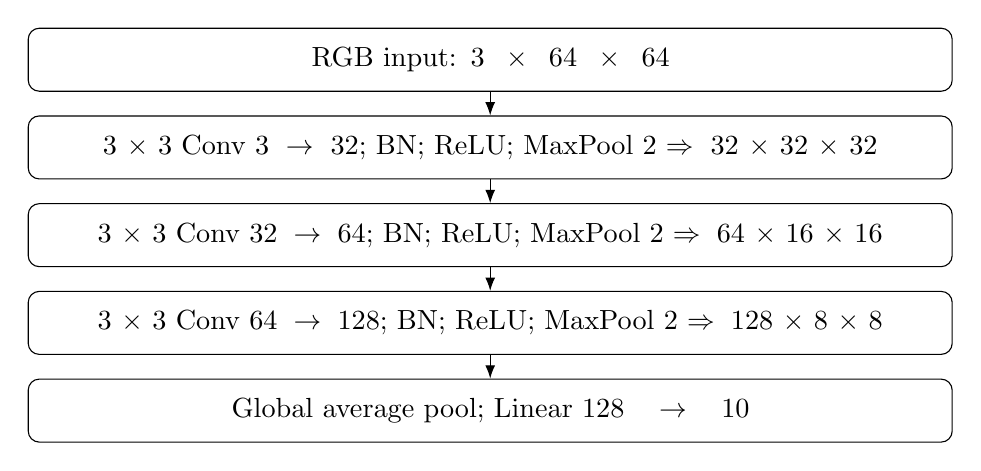
\begin{tikzpicture}[node distance=3mm,box/.style={draw,rounded corners,align=center,text width=115mm,minimum height=8mm},>=Latex]
\node[box] (a) {RGB input: $3\times64\times64$};
\node[box,below=of a] (b) {$3\times3$ Conv $3\to32$; BN; ReLU; MaxPool $2$ $\Rightarrow32\times32\times32$};
\node[box,below=of b] (c) {$3\times3$ Conv $32\to64$; BN; ReLU; MaxPool $2$ $\Rightarrow64\times16\times16$};
\node[box,below=of c] (d) {$3\times3$ Conv $64\to128$; BN; ReLU; MaxPool $2$ $\Rightarrow128\times8\times8$};
\node[box,below=of d] (e) {Global average pool; Linear $128\to10$};
\draw[->] (a)--(b);\draw[->](b)--(c);\draw[->](c)--(d);\draw[->](d)--(e);
\end{tikzpicture}\caption{Model A, drawn from the executable architecture.}\end{figure}

\subsection{Model B: depthwise-separable convolution}
The selected lightweight architecture uses three blocks with output widths 64, 128 and 256.
Each block applies a $3\times3$ depthwise convolution (one spatial filter per input channel),
then a $1\times1$ pointwise convolution, BatchNorm, ReLU and max pooling.
Both convolutions are bias-free; depthwise stride is 1 and padding is 1, while pointwise padding is 0.
Global average pooling and a biased 256-to-10 classifier complete the network.
There are no residual connections or dropout in this selected model.

\begin{figure}[htbp]\centering
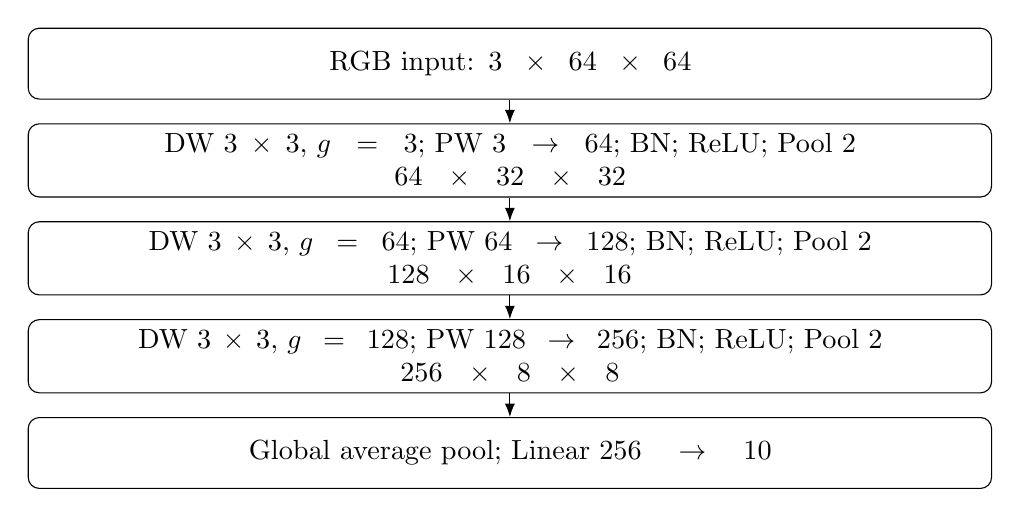
\begin{tikzpicture}[node distance=3mm,box/.style={draw,rounded corners,align=center,text width=120mm,minimum height=9mm},>=Latex]
\node[box] (a) {RGB input: $3\times64\times64$};
\node[box,below=of a] (b) {DW $3\times3$, $g=3$; PW $3\to64$; BN; ReLU; Pool $2$\\$64\times32\times32$};
\node[box,below=of b] (c) {DW $3\times3$, $g=64$; PW $64\to128$; BN; ReLU; Pool $2$\\$128\times16\times16$};
\node[box,below=of c] (d) {DW $3\times3$, $g=128$; PW $128\to256$; BN; ReLU; Pool $2$\\$256\times8\times8$};
\node[box,below=of d] (e) {Global average pool; Linear $256\to10$};
\draw[->](a)--(b);\draw[->](b)--(c);\draw[->](c)--(d);\draw[->](d)--(e);
\end{tikzpicture}\caption{Selected Model B (code \code{model_c}). DW denotes depthwise and PW denotes pointwise convolution.}\end{figure}

\subsection{Parameter calculations}
For a convolution with groups $g$, kernel $K$ and optional bias, the parameter count is
$C_{out}(C_{in}/g)K^2 + bC_{out}$, where $b=1$ if a bias is present.
Depthwise convolution has $g=C_{in}$; pointwise convolution has $K=1$.
BatchNorm contributes two trainable values per output channel. Running statistics are buffers,
not trainable parameters. A linear layer contributes $n_{in}n_{out}+n_{out}$ with a bias.

For Model A the convolutions contribute $864+18,432+73,728=93,024$ parameters;
BatchNorm adds $64+128+256=448$; the classifier adds $1,280+10=1,290$.
The total is $94,762$. For selected Model B the depthwise convolutions contribute
$27+576+1,152=1,755$, pointwise convolutions contribute $192+8,192+32,768=41,152$,
BatchNorm adds $128+256+512=896$, and the classifier adds $2,560+10=2,570$.
The total is $46,373<100,000$. Appendix tables list each executed leaf layer and check
formula totals against actual parameter tensors.

\subsection{Hardware-aware activation choice}
ReLU computes $\max(0,x)$ and requires a comparison rather than an exponential.
It is therefore a reasonable low-cost activation for the custom networks. In-place ReLU can
reuse intermediate storage when autograd permits it; this alone does not establish a peak-RAM
budget. Global average pooling avoids a large flattened fully connected head.
BatchNorm may be fused into preceding convolutions for deployment, but such fusion,
quantization and target-device execution were not measured here.

\subsection{Computational cost}
For one input, convolution MACs are
\begin{equation}\mathrm{MACs}=H_{out}W_{out}C_{out}(C_{in}/g)K^2.\end{equation}
Linear MACs are $n_{in}n_{out}$. Forward hooks independently count 41,288,960 MACs
for Model A and 18,561,536 for selected Model B at $3\times64\times64$.
These counts omit bias additions, BatchNorm, activation, pooling, residual additions,
memory access and data loading. They are not latency measurements.
For equal widths, separable convolution replaces $C_{in}C_{out}K^2$ weights with
$C_{in}K^2+C_{in}C_{out}$, but the selected model also changes widths, so the whole-network
comparison is not a matched test of convolution type alone.

\section{Optimizer selection and tuning}
\subsection{Methods and selection rule}
The saved experiments compare Adam at 0.001, plain SGD at 0.003 and 0.01, and SGD with
momentum 0.9 at 0.01, for each of three custom architectures. All run for 30 epochs.
Within each run, the checkpoint has minimum validation loss; across configurations of the same
architecture, minimum checkpoint validation loss determines the preferred configuration.
Test metrics are excluded from this rule.

Plain SGD follows a noisy negative gradient. Momentum accumulates a velocity, commonly
$v_t=\mu v_{t-1}+g_t$ and $\theta_{t+1}=\theta_t-\eta v_t$; $\mu=0.9$ retains more direction
than $\mu=0$. It can accelerate consistent descent and reduce oscillation, but may overshoot
or require a different learning rate. Adam uses bias-corrected first and second gradient moments
to adapt the update scale~\cite{adam}. The recorded Adam learning rate is lower than the
momentum-SGD rate, so differences cannot be attributed to momentum alone across all methods.

\subsection{Observed experiments}
\begin{table}[htbp]\centering\small
\resizebox{\linewidth}{!}{\begin{tabular}{lrrrrrrr}
\toprule
Code & Optimizer & LR & Mom. & Epoch & Val. loss & Val. acc. (\%) & Train s \\
\midrule
model\_a & adam & 0.001 & 0 & 30 & 0.1721 & 94.12 & 26.78 \\
model\_a & sgd & 0.003 & 0 & 29 & 0.4595 & 83.63 & 28.10 \\
model\_a & sgd & 0.01 & 0 & 27 & 0.3796 & 87.21 & 26.01 \\
model\_a & sgd\_momentum & 0.01 & 0.9 & 30 & 0.1745 & 94.20 & 23.94 \\
model\_b & adam & 0.001 & 0 & 27 & 0.2445 & 91.56 & 27.79 \\
model\_b & sgd & 0.003 & 0 & 28 & 0.6512 & 78.30 & 27.93 \\
model\_b & sgd & 0.01 & 0 & 28 & 0.4831 & 83.53 & 25.39 \\
model\_b & sgd\_momentum & 0.01 & 0.9 & 25 & 0.2347 & 91.83 & 26.10 \\
model\_c & adam & 0.001 & 0 & 28 & 0.1776 & 94.00 & 30.53 \\
model\_c & sgd & 0.003 & 0 & 29 & 0.5881 & 79.60 & 24.33 \\
model\_c & sgd & 0.01 & 0 & 29 & 0.4166 & 85.01 & 34.29 \\
model\_c & sgd\_momentum & 0.01 & 0.9 & 29 & 0.2183 & 92.32 & 25.92 \\
\bottomrule
\end{tabular}
}
\caption{Each row uses the minimum-validation-loss epoch. Train s is mean training-pass time over all 30 epochs; validation time is excluded. Historical code labels are retained.}\end{table}
\fig{optimizer_comparison.pdf}{1}{Validation accuracy at the selected epoch. The earliest lightweight baseline is code \code{model_b}; it is not the final selected Model B.}

Adam 0.001 gives the lowest recorded validation loss for Model A and \code{model_c}.
For the initial \code{model_b}, momentum SGD 0.01 gives the lowest loss.
Momentum SGD substantially improves on plain SGD 0.01 within this 30-epoch budget.
For Model A, momentum SGD has slightly higher selected validation accuracy than Adam,
but Adam has lower validation loss, so Adam remains selected. Model B's wider channels
recover validation performance relative to the initial lightweight baseline while staying
below the parameter cap. One seed and a small learning-rate grid do not establish a universal
optimizer ranking; neither optimizer family was exhaustively tuned.

\section{Custom model training and evaluation}
\subsection{Training setup and learning curves}
The final custom runs use seed 42, batch size 64, Adam 0.001, weight decay 0.0001 and
30 epochs, satisfying the minimum-20-epoch requirement. The pipeline is FP32 cross-entropy
with no learning-rate scheduler or early stopping. The selected epochs are 30 for Model A
and 28 for selected Model B. Saved configurations identify CUDA; historical training timings
come from the recorded machine, not this CPU cloud environment.
\fig{model_a_curves.pdf}{1}{Model A training/validation history. The dotted line identifies the minimum-validation-loss epoch.}
\fig{model_c_curves.pdf}{1}{Selected Model B training/validation history. Curves are raw saved values, not smoothed estimates.}

\subsection{Test metrics and storage}
The four saved prediction files contain the same 4,050 test filenames and true labels in the
same order. Confusion matrices, precision, recall, F1 and overall accuracy were recomputed
from these files and matched the saved reports within $10^{-12}$.
This is an audit of saved predictions, not new test inference from trained checkpoints.
\begin{table}[htbp]\centering\small\resizebox{\linewidth}{!}{\begin{tabular}{lrrrrr}
\toprule
Model & Params & FP32 KB & Weights KB* & Train s & Test \% \\
\midrule
Standard A & 94,762 & 379.048 & 387.218 & 26.78 & 93.90 \\
Selected lightweight B & 46,373 & 185.492 & 196.521 & 30.53 & 94.37 \\
\bottomrule
\end{tabular}
}
\caption{Custom-model comparison. KB is 1,000 bytes. FP32 KB counts trainable parameter tensors only. *Weights KB is the historical serialized-file measurement recorded in metrics; the trained files are absent for remeasurement.}\end{table}

Selected Model B's test accuracy exceeds Model A's by approximately 0.47 percentage points
(19 more correct predictions). This is a descriptive result on one split, not evidence of
statistically robust superiority. The selected lightweight model halves parameter storage
approximately and reduces convolution/linear computation, but its mean recorded training
time is not lower. Implementation, kernel utilization, startup, data loading and shared-machine
conditions can dominate wall-clock measurements.

\subsection{Confusion matrices and class performance}
\fig{model_a_confusion.pdf}{.86}{Model A test confusion matrix recalculated from saved predictions. Rows are true classes, columns predicted classes.}
\fig{model_c_confusion.pdf}{.86}{Selected Model B test confusion matrix recalculated from saved predictions.}
Macro precision and recall weight the ten classes equally. Overall accuracy weights images;
it can conceal lower recall for smaller classes. The full per-class tables in the appendix
avoid treating overall accuracy as a complete error characterization. Confusions among
agricultural/vegetation classes are plausible at this spatial resolution, but these matrices
do not establish which visual features caused individual errors.

\section{Lightweight pretrained architectures}
\subsection{MobileNetV2 and ShuffleNetV2 x0.5}
MobileNetV2 uses inverted residual blocks with expansion, depthwise filtering and linear
bottlenecks~\cite{mobilenetv2}. ShuffleNetV2 uses channel split/shuffle and efficient branches;
its design also considers practical execution cost beyond arithmetic counts~\cite{shufflenetv2}.
The x0.5 variant has fewer channels than larger ShuffleNetV2 versions.

The executable loader first builds the original 1,000-class model, loads the official ImageNet
state, and only then replaces the classifier with ten outputs. All layers remain trainable.
MobileNetV2 uses \code{MobileNet_V2_Weights.IMAGENET1K_V2}; ShuffleNetV2 uses
\code{ShuffleNet_V2_X0_5_Weights.IMAGENET1K_V1}~\cite{torchvision}.
Source-file SHA-256 prefixes and strict state dictionaries are checked, including cached/manual
sources. Loading failure raises an error instead of falling back to random initialization.

During this audit, genuine official sources were hash-verified and synthetic tests checked
backbone initialization and updates. Historical run configs also record successful pretrained
initialization and full source hashes. This supports the intended training provenance; without
the historical trained checkpoints, the exact final weight trajectories cannot be reverified.

\subsection{Fine-tuning protocol and results}
Both fine-tuning runs use the same saved split fingerprints, batch size 64, seed 42,
30 epochs, Adam 0.0001 and weight decay 0.0001. Minimum validation loss selects
epochs 27 (MobileNetV2) and 29 (ShuffleNetV2). Inputs stay at 64-by-64 rather than the
larger default ImageNet evaluation size. ImageNet normalization is the documented exception
to the custom preprocessing. No claim of matching published ImageNet benchmarks is made.
\fig{mobilenet_v2_curves.pdf}{1}{MobileNetV2 saved fine-tuning history.}
\fig{shufflenet_v2_x0_5_curves.pdf}{1}{ShuffleNetV2 x0.5 saved fine-tuning history.}

\section{Final comparison and trade-offs}
\begin{table}[htbp]\centering\scriptsize
\resizebox{\linewidth}{!}{\begin{tabular}{lrrrrrrrrr}
\toprule
Model & Params & Weights MB* & MACs M & Val. \% & Test \% & Prec. \% & Recall \% & F1 \% & Train s \\
\midrule
Standard A & 94,762 & 0.387218 & 41.289 & 94.12 & 93.90 & 93.90 & 93.70 & 93.75 & 26.78 \\
Selected lightweight B & 46,373 & 0.196521 & 18.562 & 94.00 & 94.37 & 94.23 & 94.25 & 94.18 & 30.53 \\
Model D & 15,442 & 0.082062 & 4.729 & 94.17 & 93.63 & 93.43 & 93.42 & 93.40 & 21.23 \\
MobileNetV2 & 2,236,682 & 9.180270 & 24.461 & 98.02 & 98.12 & 98.11 & 97.95 & 98.02 & 42.16 \\
ShuffleNetV2 x0.5 & 352,042 & 1.542078 & 3.231 & 96.20 & 96.37 & 96.21 & 96.23 & 96.21 & 37.26 \\
\bottomrule
\end{tabular}
}
\caption{Verified saved-prediction comparison and source-derived costs. Precision, recall and F1 are macro averages. Validation accuracy is at minimum validation loss. *Weight size is recorded, not remeasured. Mean train seconds excludes validation but includes the first epoch.}\end{table}
\fig{final_comparison.pdf}{1}{Accuracy, recorded serialized storage (log scale) and convolution/linear computation. These are complementary criteria; no panel measures edge latency.}

\subsection{Accuracy}
MobileNetV2 has the highest saved test accuracy (98.12\%), followed by ShuffleNetV2 x0.5
(96.37\%), selected Model B (94.37\%) and Model A (93.90\%). Pretraining provides a useful
starting representation and increases accuracy in these experiments. Because architecture,
initialization, normalization and learning rate differ, this is not a causal ablation of
pretraining alone. All figures describe a single split and seed; small differences should not
be generalized as stable rankings without repeated runs.

\subsection{Memory footprint and computation}
Selected Model B has the smallest parameter count and recorded weight file among the four
required models: 46,373 parameters and 0.196521 MB. MobileNetV2 uses approximately 48.2 times
as many parameters; ShuffleNetV2 uses 7.6 times as many. Serialized files include BatchNorm
buffers and serialization overhead in addition to parameter tensors; training resume files
also include optimizer and random-generator state. None of these sizes is peak inference RAM.

ShuffleNetV2 has the lowest counted computation among the required models: 3.231 million
MACs/image, compared with 18.562 million for selected Model B. Thus the smallest parameter
model is not necessarily the lowest-compute model. Channel widths, feature resolutions and
layer arrangement matter. Memory traffic, operator fusion and hardware kernels also affect
latency, so a MAC ranking cannot replace a device benchmark.

\fig{parameter_storage.pdf}{1}{Parameters and storage. The raw FP32 parameter estimate and the recorded serialized state-dictionary size describe different storage scopes. Neither is peak RAM.}

\subsection{Training time and deployment implications}
\begin{table}[htbp]\centering\small\begin{tabular}{lrrr}
\toprule
Model & Mean s & Mean excl. first s & Test pass s \\
\midrule
Standard A & 26.777 & 25.267 & 42.741 \\
Selected lightweight B & 30.532 & 25.624 & 3.463 \\
MobileNetV2 & 42.158 & 36.505 & 4.113 \\
ShuffleNetV2 x0.5 & 37.264 & 31.275 & 3.711 \\
\bottomrule
\end{tabular}

\caption{Recorded timings, in seconds. Test pass time includes loading, transfers, loss and prediction collection, with CUDA synchronization; it is not model-only latency.}\end{table}
Reporting means with and without the first epoch exposes startup sensitivity; it does not
make timings comparable to an edge target. Under a strict storage limit, the custom selected
Model B is attractive. When accuracy dominates and memory permits, MobileNetV2 is attractive.
ShuffleNetV2 offers the lowest counted computation with intermediate storage. A final device
choice still requires target latency, peak RAM, energy, quantization calibration and robustness
measurements. These were not measured here.

\section{Additional architecture audit}
\subsection{CompactEuroSAT candidate}
The \code{simple_model} branch contains a compact CNN with a standard $3\times3$ stem
($3\to16$), then depthwise-separable blocks $16\to32$ (stride 2), $32\to48$ (stride 2),
$48\to48$ (stride 1, identity residual) and $48\to80$ (stride 2).
Each depthwise stage uses a $3\times3$ kernel, padding 1, no bias and channel-wise grouping;
pointwise stages use $1\times1$ kernels and no bias. Both stages have BatchNorm, with ReLU
after depthwise normalization and after the block. Global average pooling, dropout 0.10
and a biased 80-to-10 linear layer form the head. Source-derived cost is 11,466 parameters,
45,864 FP32 parameter bytes, and 3,882,784 convolution/linear MACs per image.

The historical notebook prints 94.716\% test accuracy and approximately 94.64\% validation
accuracy. These are saved notebook claims, not a new verified controlled result. Reconstruction
of its sorted-folder, stratified seed-42 split exactly matches the canonical memberships;
the actual historical manifest files and trained checkpoint are not committed, so the
reconstruction does not prove what files existed on the Kaggle machine.
Its optimizer protocol differs: batch size 128, maximum 60 epochs, patience 12,
cosine scheduling, colour jitter, gradient clipping, CUDA mixed precision, no Adam weight
decay argument, and checkpoint selection by validation macro-F1. Consequently its higher
printed accuracy is not used to select a replacement Model B.

The historical notebook and duplicate \code{lightweight_CNN} file remain unchanged.
A shared-CLI implementation is tested for exact evaluation-output equivalence after state
loading, forward shapes and a real synthetic optimizer step. A controlled new run is prepared
with the common manifests, 30 epochs, seed 42, batch 64, Adam 0.001, weight decay 0.0001,
shared augmentation/normalization and minimum-validation-loss selection. Missing RGB files
and blocked official download routes prevented execution. Its controlled validation/test
metrics, timing and actual trained-file size are therefore \textbf{not available}.

The candidate's resource costs are promising, but no recommendation to replace selected
Model B is justified before validation under the controlled protocol. Repeated selection
against known test results would contaminate the test set; any further search should use
validation data and ideally a genuinely held-out confirmation dataset.

\subsection{ResidualDepthwiseCNN (Model D)}
Branch \code{nipun} adds a 24-channel standard stem and residual depthwise blocks
$24\to24$, $24\to48$ and $48\to96$, each downsampling by stride 2, then global average
pooling and a 96-to-10 classifier. Independent execution of its architecture definitions gives
15,442 parameters and 4,728,768 convolution/linear MACs per input. The branch's Markdown
claims 93.63\% test accuracy, but its Model D config, history, predictions, confusion matrix
and trained checkpoint are not committed. Its split hashes are consistent with CRLF versions
of the canonical CSVs, but a prose claim is insufficient to verify an experiment.
Model D is therefore an optional architecture audit, excluded from the verified master table.
No matched residual/non-residual ablation exists; residual connections cannot be credited
causally for any claimed performance change.

\section{Conclusion}
The selected custom Model B meets the 100,000-parameter cap and preserves useful accuracy
with substantially lower parameter storage and counted computation than Model A.
The saved four-model comparison highlights complementary strengths: MobileNetV2 prioritizes
accuracy, ShuffleNetV2 has the lowest counted arithmetic, and the custom selected model
has the smallest recorded storage. The data do not identify a universally best edge model.
CompactEuroSAT and Model D merit further validation but do not justify a test-driven model
replacement. The current report is editable and its tables trace to repository artifacts;
name spelling, dataset-sheet status and missing experiment artifacts remain explicit checks
before submission.

\bibliographystyle{plainnat}
\bibliography{references}
\clearpage\appendix
\section{Detailed layer calculations}
\subsection{Model A}
\begin{table}[H]\centering\scriptsize\resizebox{\linewidth}{!}{\begin{tabular}{lrrr}
\toprule
Operation & Output C x H x W & Formula & Params \\
\midrule
Conv2d k3 s1 p1 g1 & 32 x 64 x 64 & 32 x 3 x 3 x 3 + 0 & 864 \\
BatchNorm2d & 32 x 64 x 64 & 2 x 32 & 64 \\
ReLU & 32 x 64 x 64 & 0 & 0 \\
MaxPool2d & 32 x 32 x 32 & 0 & 0 \\
Conv2d k3 s1 p1 g1 & 64 x 32 x 32 & 64 x 32 x 3 x 3 + 0 & 18,432 \\
BatchNorm2d & 64 x 32 x 32 & 2 x 64 & 128 \\
ReLU & 64 x 32 x 32 & 0 & 0 \\
MaxPool2d & 64 x 16 x 16 & 0 & 0 \\
Conv2d k3 s1 p1 g1 & 128 x 16 x 16 & 128 x 64 x 3 x 3 + 0 & 73,728 \\
BatchNorm2d & 128 x 16 x 16 & 2 x 128 & 256 \\
ReLU & 128 x 16 x 16 & 0 & 0 \\
MaxPool2d & 128 x 8 x 8 & 0 & 0 \\
AdaptiveAvgPool2d & 128 x 1 x 1 & 0 & 0 \\
Linear & 10 & 128 x 10 + 10 & 1,290 \\
\bottomrule
\end{tabular}
}
\caption{Executed leaf layers of Model A. Group $g$, stride $s$, padding $p$ and kernel $k$ are explicit. Outputs exclude the batch dimension.}\end{table}
\subsection{Selected Model B}
\begin{table}[H]\centering\scriptsize\resizebox{\linewidth}{!}{\begin{tabular}{lrrr}
\toprule
Operation & Output C x H x W & Formula & Params \\
\midrule
Conv2d k3 s1 p1 g3 & 3 x 64 x 64 & 3 x 1 x 3 x 3 + 0 & 27 \\
Conv2d k1 s1 p0 g1 & 64 x 64 x 64 & 64 x 3 x 1 x 1 + 0 & 192 \\
BatchNorm2d & 64 x 64 x 64 & 2 x 64 & 128 \\
ReLU & 64 x 64 x 64 & 0 & 0 \\
MaxPool2d & 64 x 32 x 32 & 0 & 0 \\
Conv2d k3 s1 p1 g64 & 64 x 32 x 32 & 64 x 1 x 3 x 3 + 0 & 576 \\
Conv2d k1 s1 p0 g1 & 128 x 32 x 32 & 128 x 64 x 1 x 1 + 0 & 8,192 \\
BatchNorm2d & 128 x 32 x 32 & 2 x 128 & 256 \\
ReLU & 128 x 32 x 32 & 0 & 0 \\
MaxPool2d & 128 x 16 x 16 & 0 & 0 \\
Conv2d k3 s1 p1 g128 & 128 x 16 x 16 & 128 x 1 x 3 x 3 + 0 & 1,152 \\
Conv2d k1 s1 p0 g1 & 256 x 16 x 16 & 256 x 128 x 1 x 1 + 0 & 32,768 \\
BatchNorm2d & 256 x 16 x 16 & 2 x 256 & 512 \\
ReLU & 256 x 16 x 16 & 0 & 0 \\
MaxPool2d & 256 x 8 x 8 & 0 & 0 \\
AdaptiveAvgPool2d & 256 x 1 x 1 & 0 & 0 \\
Linear & 10 & 256 x 10 + 10 & 2,570 \\
\bottomrule
\end{tabular}
}
\caption{Executed leaf layers of selected Model B. All zero-parameter pooling/activation stages are included.}\end{table}
\clearpage
\section{Per-class saved test metrics}
\begin{table}[H]\centering\small\begin{tabular}{lrrrr}
\toprule
Class & Precision & Recall & F1 & Support \\
\midrule
AnnualCrop & 0.9591 & 0.8867 & 0.9215 & 450 \\
Forest & 0.9718 & 0.9956 & 0.9835 & 450 \\
HerbaceousVegetation & 0.8884 & 0.9556 & 0.9208 & 450 \\
Highway & 0.9542 & 0.8880 & 0.9199 & 375 \\
Industrial & 0.9750 & 0.9360 & 0.9551 & 375 \\
Pasture & 0.9439 & 0.9533 & 0.9486 & 300 \\
PermanentCrop & 0.8564 & 0.8907 & 0.8732 & 375 \\
Residential & 0.9468 & 0.9889 & 0.9674 & 450 \\
River & 0.9079 & 0.8933 & 0.9005 & 375 \\
SeaLake & 0.9866 & 0.9822 & 0.9844 & 450 \\
\bottomrule
\end{tabular}
\caption{Model A.}\end{table}
\begin{table}[H]\centering\small\begin{tabular}{lrrrr}
\toprule
Class & Precision & Recall & F1 & Support \\
\midrule
AnnualCrop & 0.9246 & 0.9267 & 0.9256 & 450 \\
Forest & 0.9823 & 0.9889 & 0.9856 & 450 \\
HerbaceousVegetation & 0.9087 & 0.9289 & 0.9187 & 450 \\
Highway & 0.9556 & 0.8613 & 0.9060 & 375 \\
Industrial & 0.9634 & 0.9813 & 0.9723 & 375 \\
Pasture & 0.9128 & 0.9767 & 0.9436 & 300 \\
PermanentCrop & 0.9200 & 0.8587 & 0.8883 & 375 \\
Residential & 0.9866 & 0.9800 & 0.9833 & 450 \\
River & 0.8819 & 0.9360 & 0.9082 & 375 \\
SeaLake & 0.9867 & 0.9867 & 0.9867 & 450 \\
\bottomrule
\end{tabular}
\caption{Selected Model B.}\end{table}
\begin{table}[H]\centering\small\begin{tabular}{lrrrr}
\toprule
Class & Precision & Recall & F1 & Support \\
\midrule
AnnualCrop & 0.9692 & 0.9800 & 0.9746 & 450 \\
Forest & 0.9868 & 0.9978 & 0.9923 & 450 \\
HerbaceousVegetation & 0.9758 & 0.9867 & 0.9812 & 450 \\
Highway & 0.9812 & 0.9733 & 0.9772 & 375 \\
Industrial & 0.9892 & 0.9733 & 0.9812 & 375 \\
Pasture & 0.9727 & 0.9500 & 0.9612 & 300 \\
PermanentCrop & 0.9781 & 0.9520 & 0.9649 & 375 \\
Residential & 0.9782 & 0.9978 & 0.9879 & 450 \\
River & 0.9866 & 0.9840 & 0.9853 & 375 \\
SeaLake & 0.9934 & 1.0000 & 0.9967 & 450 \\
\bottomrule
\end{tabular}
\caption{MobileNetV2.}\end{table}
\begin{table}[H]\centering\small\begin{tabular}{lrrrr}
\toprule
Class & Precision & Recall & F1 & Support \\
\midrule
AnnualCrop & 0.9510 & 0.9489 & 0.9499 & 450 \\
Forest & 0.9781 & 0.9933 & 0.9857 & 450 \\
HerbaceousVegetation & 0.9600 & 0.9600 & 0.9600 & 450 \\
Highway & 0.9288 & 0.9387 & 0.9337 & 375 \\
Industrial & 0.9813 & 0.9813 & 0.9813 & 375 \\
Pasture & 0.9385 & 0.9667 & 0.9524 & 300 \\
PermanentCrop & 0.9322 & 0.9173 & 0.9247 & 375 \\
Residential & 0.9911 & 0.9933 & 0.9922 & 450 \\
River & 0.9667 & 0.9280 & 0.9469 & 375 \\
SeaLake & 0.9933 & 0.9956 & 0.9945 & 450 \\
\bottomrule
\end{tabular}
\caption{ShuffleNetV2 x0.5.}\end{table}

\section{Reproducibility and audit limits}\label{sec:repro}
The artifact generator \code{report/generate.py} checks manifests, reconstructs compact split
membership, recomputes all final classification metrics, checks per-class and confusion files,
recalculates parameter/MAC counts, and creates figures directly from histories/predictions.
\code{report/audit/report_data_sources.csv} maps generated values to their source files and
evidence level. Model-layer CSVs include operation dimensions, formulas, parameter counts
and MACs. Recorded file sizes are not silently relabelled as new measurements.

The four canonical final reports are in timestamped \code{outputs/reports/evaluate-test_*}
directories. Their configurations and histories identify the source run names. The raw Git
CSV bytes use LF line endings, whereas the historical saved split and source hashes match
CRLF serializations. This was verified in memory without altering files or expected hashes.
Two final-audit test methods fail for this byte-level difference. The existing evaluation CLI
also checks literal split fingerprints; replaying a Windows run on an LF checkout needs an
explicit, audited portability change or a separate matching serialization, not a changed
expected hash. Historical exact-resume additionally requires the recorded device, workers,
Python and package versions and full optimizer/RNG checkpoints.

The source branch audit uses fetched remote refs. Dataset/setup/standard-CNN/integration branches
are already ancestors of main; \code{heshan} equals main. \code{simple_model} was 18 commits ahead
and 19 behind; it was synchronized with a normal merge after creating safety branches.
\code{nipun} is three commits ahead of main and remains separate. Main was not modified.
Repository history begins on 10 September 2026 and includes later dataset, model and integration
commits; the visible history is preserved rather than manufactured for submission.

\begin{longtable}{p{.58\linewidth}p{.34\linewidth}}\toprule
Requirement / reproducibility item & Audit outcome\\\midrule\endhead
Assignment PDF read & Supplied filename differs from request; contents read.\\
Dataset source, RGB, $64\times64$ & Documented; loader enforces shape; raw images absent.\\
70/15/15 splits, saved filenames/class order & Verified from manifests; no overlapping paths/hashes.\\
Normalization and augmentation & Verified from source/configs; no statistics recalculated.\\
Seed, optimizer, LR, batch size, epochs & Saved configs/histories inspected; one seed each.\\
Checkpoint selection & Minimum validation loss in source/history; historical checkpoints absent.\\
Model A standard conv/max pooling & Verified from executable source.\\
Model B depthwise and parameter cap & 46,373 parameters, independently verified.\\
Activation/hardware justification & ReLU explained; hardware speed not measured.\\
Optimizer comparisons and momentum & Twelve saved runs checked.\\
At least 20 custom training epochs & Thirty rows per saved run; no new retraining claim.\\
Test metrics and confusion matrices & Recomputed from four saved prediction files.\\
Model size and time comparison & Recorded sizes/timings labelled; files absent.\\
Two genuine pretrained mobile models & Official initialization tested; historical configs checked.\\
Accuracy/memory/computation discussion & Included; latency/RAM/energy unmeasured.\\
Controlled CompactEuroSAT evaluation & Blocked by missing images / download-route 403.\\
Model D optional result verification & Architecture verified; result artifacts unavailable.\\
Dataset assignment sheet update & External sheet status unknown; group action required.\\
Group number and names & Group 54 supplied by user; names agree in Git, spelling confirmation required.\\
GitHub/profile link and history & Included; original history preserved.\\
Report/code separate Moodle submission & Not performed; group must submit once.\\
\bottomrule\end{longtable}
\end{document}
